\documentclass[11pt]{resume} % Use the custom resume.cls style - 11pt is standard

\usepackage[left=0.4in, top=0.4in, right=0.4in, bottom=0.4in]{geometry} % Keep tight margins
\usepackage[normalem]{ulem} % For \uline
\usepackage{enumitem}     % For list spacing control
\usepackage{hyperref}
\hypersetup{colorlinks=true, linkcolor=blue, urlcolor=blue} % Optional: color links
\usepackage{amsmath} % For \textsubscript if needed, and general math symbols
\usepackage{graphicx} % For including images
\usepackage[absolute,overlay]{textpos} % For precise image positioning
\usepackage{hyperref} % For clickable links (already likely included)
\usepackage{calc}     % May be needed for calculations with lengths like \textwidth


% Your custom commands (keep if needed by resume.cls)
\newcommand{\tab}[1]{\hspace{.2667\textwidth}\rlap{#1}}
\newcommand{\itab}[1]{\hspace{0em}\rlap{#1}}

% Textpos configuration for image placement
\setlength{\TPHorizModule}{1mm} % Use millimeters as units for positioning
\setlength{\TPVertModule}{1mm}
\newcommand{\imagewidth}{30} % Set your desired image width in mm
\newcommand{\imageoffset}{5} % Right margin offset in mm
\newcommand{\topoffset}{5}   % Top margin offset in mm

% \name{WARIT YUVANIYAMA (NOTE)} % Using all caps can look cleaner for names
% % Using multiple address commands to control layout based on resume.cls behavior
% \address{Second Year Computer Engineering Student}
% \address{Sirindhorn International Institute of Technology (SIIT), Thammasat University}
% \address{ % Contact Info Line
%     \href{tel:+66959638282(Thailand)}{+66 9596 38282} \textbf{ | } % Use \textbf{ | } for consistent spacing
%     \href{mailto:6622770459@g.siit.tu.ac.th}{6622770459@g.siit.tu.ac.th} \textbf{ | }
%     \href{https://www.linkedin.com/in/warit-yuvaniyama-897194257/}{LinkedIn} \textbf{ | }
%     \href{https://github.com/Warit-Yuv}{GitHub}
% }

% Global list settings for compactness (adjust itemsep as needed, e.g., -3pt)
\setlist{itemsep=-2pt, topsep=1pt, parsep=0pt, partopsep=0pt}

\begin{document}

% --- Picture Block (Top Right Corner) ---
\begin{textblock*}{\imagewidth mm}(\textwidth - \imagewidth mm - \imageoffset mm + \hoffset + 12.5mm, \topoffset mm + \voffset) % Calculate X, Y position
   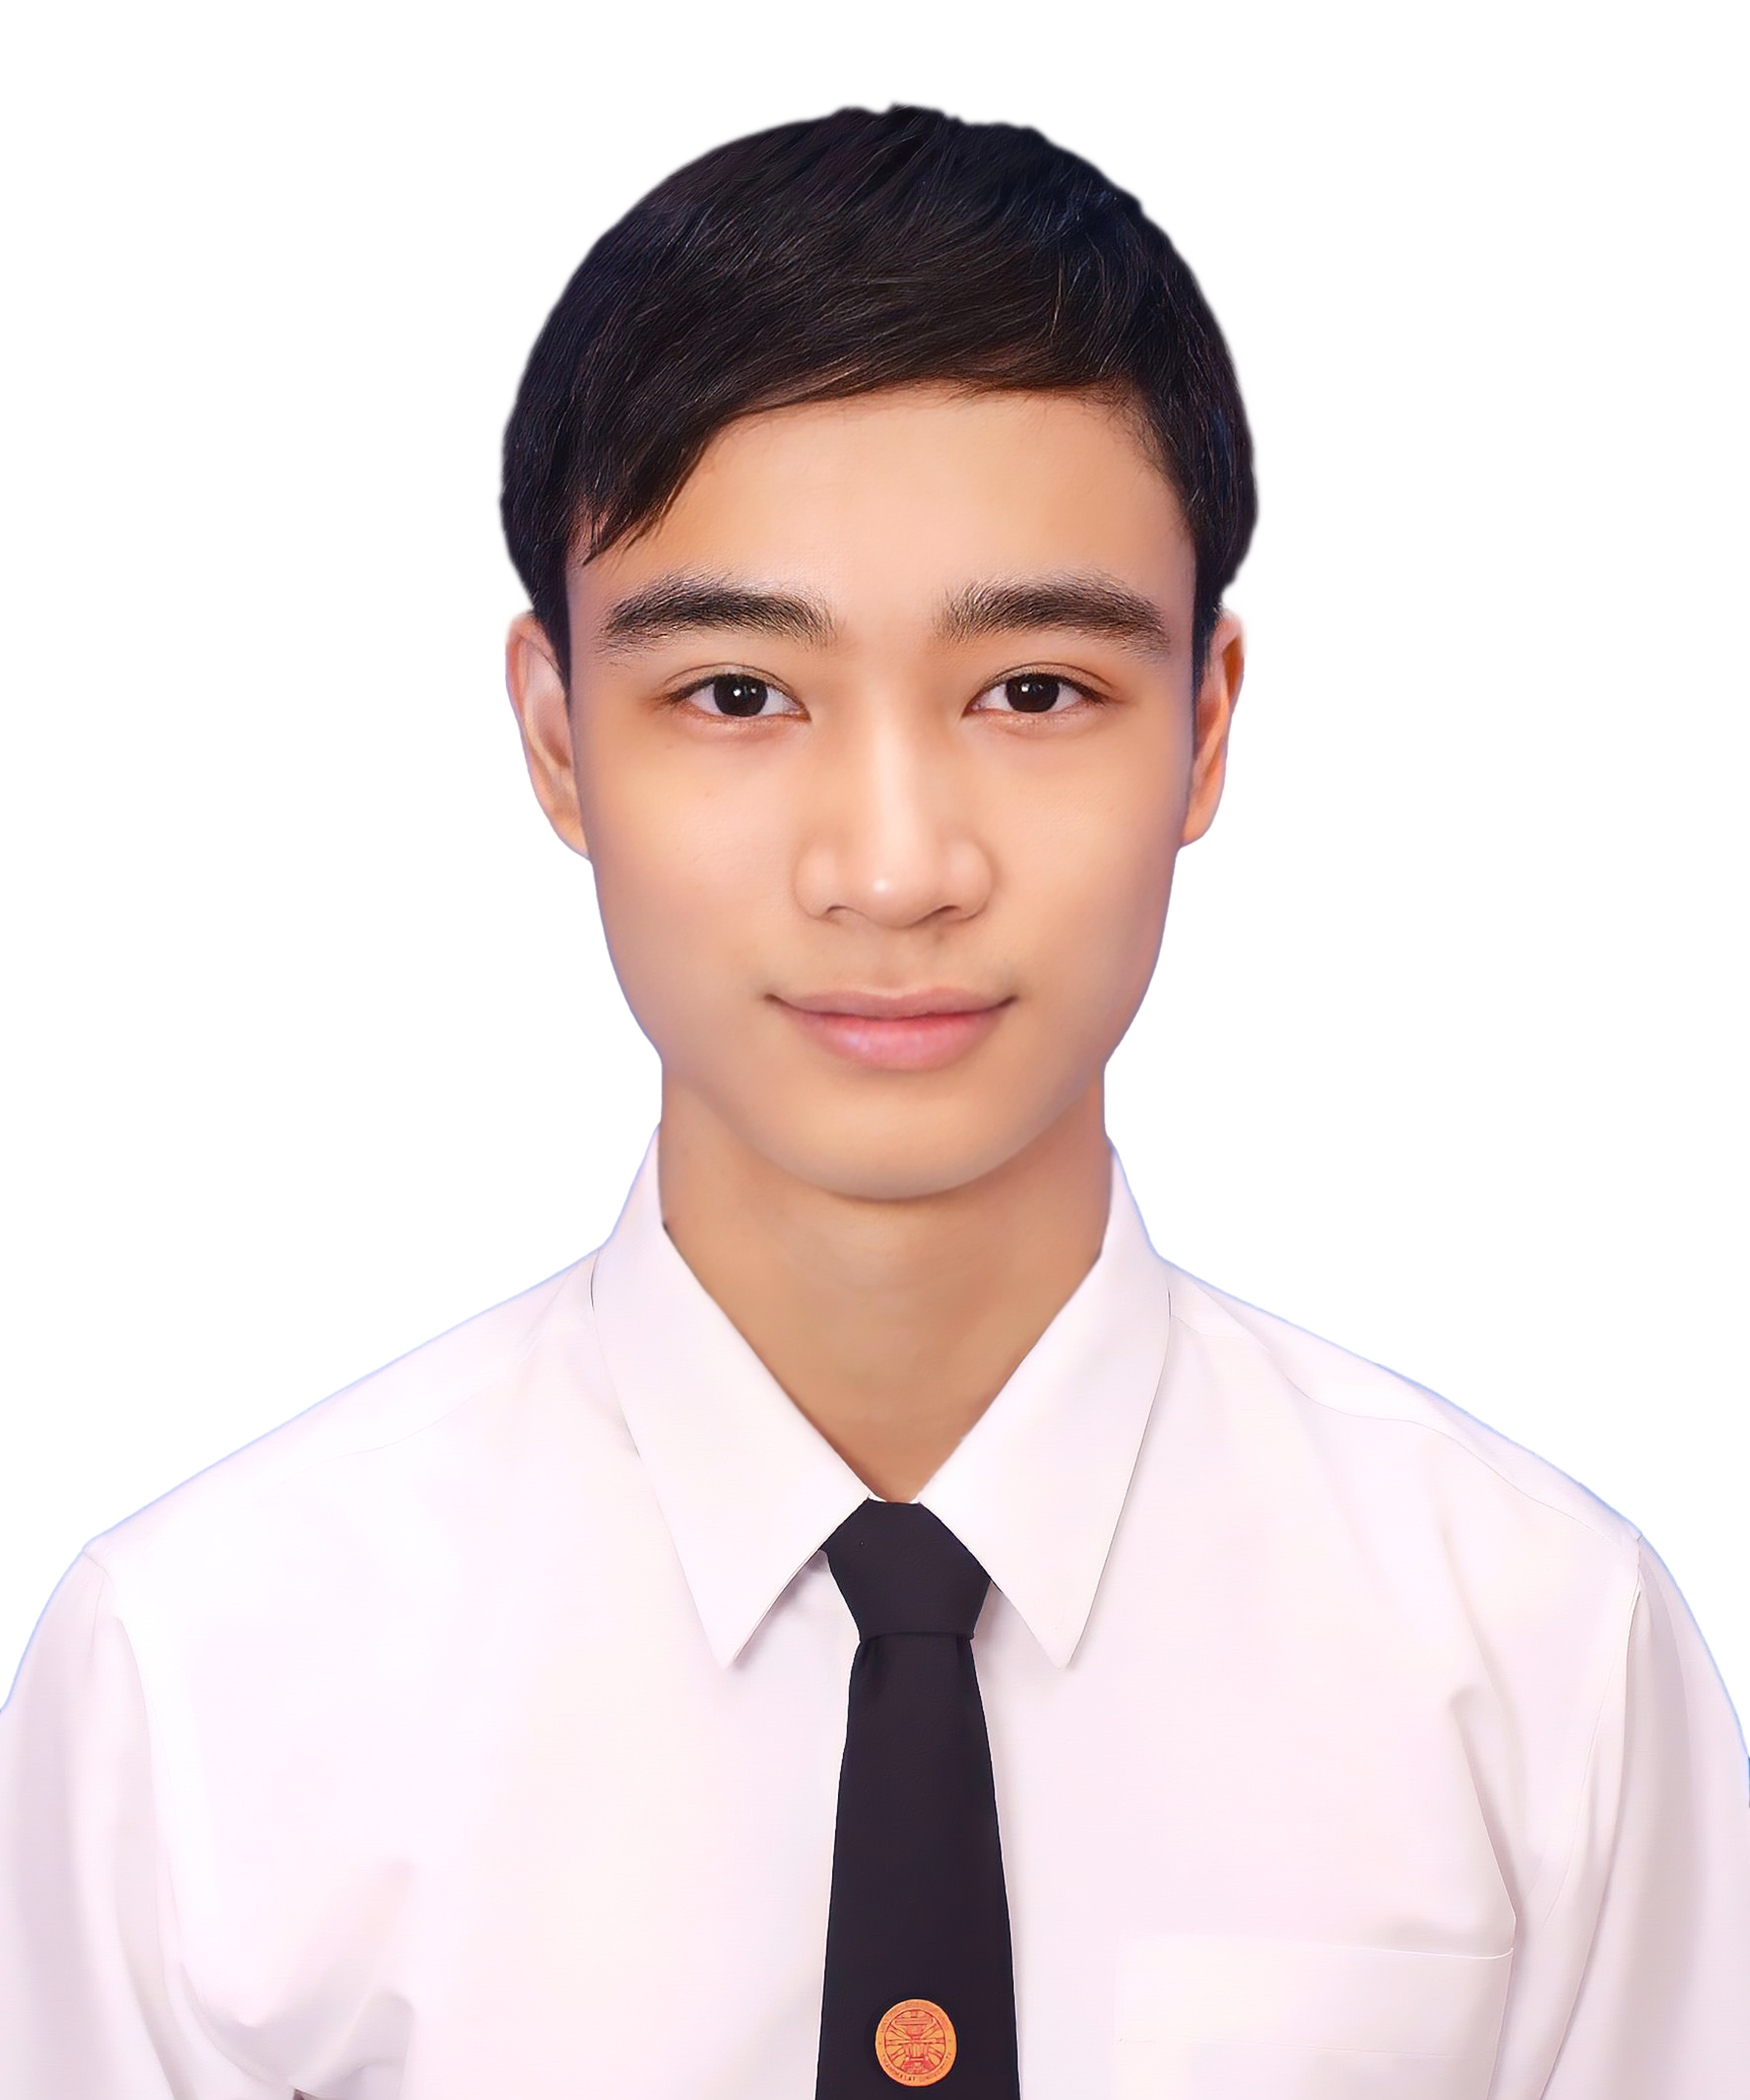
\includegraphics[width=\imagewidth mm]{6622770459 - transparent.png}
\end{textblock*}

% --- Header Text Block (Shifted Left) ---
\noindent % Prevent paragraph indentation
\hspace*{-2mm}% <--- Adjust this negative value to shift the text block LEFTWARDS
\begin{minipage}[t]{0.8\textwidth} % Adjust width (e.g., 0.8\textwidth) as needed; [t] aligns the top
    \centering % Center text within this minipage block
    {\LARGE \bfseries WARIT YUVANIYAMA (NOTE)} \\[.8ex] % Name
    {\normalsize % Font size for contact/address lines
        \href{tel:+66959638282}{+66 9596 38282} \textbf{ | }
        \href{mailto:6622770459@g.siit.tu.ac.th}{6622770459@g.siit.tu.ac.th} \textbf{ | }
        \href{https://www.linkedin.com/in/warit-yuvaniyama/}{LinkedIn} \textbf{ | }
        \href{https://github.com/Warit-Yuv}{GitHub}
    } \\[.5ex] % Small space after contact info
    {\large Third Year Computer Engineering Student} \\ % Address line 1
    {\large Sirindhorn International Institute of Technology (SIIT), Thammasat University} % Address line 2
\end{minipage}% Note the '%' sign here to prevent unwanted space after minipage
\par % End the paragraph to ensure proper spacing below
\vspace{1em} % Add vertical space below the header block before the first section

%----------------------------------------------------------------------------------------
% SUMMARY SECTION
%----------------------------------------------------------------------------------------
\begin{rSection}{SUMMARY}
High-achieving Computer Engineering student (3.98 CGPA) and President of SIIT Academy Club (OrcaBOT). \\ Proficient in \textbf{embedded systems design} using \textbf{C++, Python, and ROS2}, with peer-reviewed research publications. Proven leader in managing technical procurement (budgeting \textbf{100,000+ THB}) and an award-winning communicator with a track record in technical pitching for innovative solutions in Sustainability and Smart Cities.
\end{rSection}

%----------------------------------------------------------------------------------------
% EDUCATION SECTION
%----------------------------------------------------------------------------------------
\vspace{-1mm} % Adjust slightly if needed
\begin{rSection}{Education}
    {\bf Bachelor of Computer Engineering}, SIIT, Thammasat University \hfill {Expected 2027} \\
    CGPA: 3.98 (Expected First-Class Honors); Recipient of Academic Outstanding Student Scholarship.
    \begin{itemize}[leftmargin=*, itemsep=-3pt, topsep=-5pt]
        \item \textit{Relevant Coursework:} Microcontrollers \& Applications, Circuit Analysis, Database Systems, Operating Systems, Computer Architecture, Artificial Intelligence \& Applications, Object-Oriented Programming, Algorithm Design. % Use one line if it fits nicely
    \end{itemize}
    \vspace{0.25em}

    {\bf High School (DPSTE Program)}, Samsenwittayalai School \hfill {Graduated Feb 2023} \\
    CGPA: 3.96
     \begin{itemize}[leftmargin=*, itemsep=-3pt, topsep=-5pt]
        \item \textit{Relevant Coursework:} Computer and Algorithm, Programming, Introduction to Research Methodology, \\Design and Technology, Science Project, English for Academic Purpose.
     \end{itemize}
\end{rSection}

%----------------------------------------------------------------------------------------
% SKILLS SECTION
%----------------------------------------------------------------------------------------
\vspace{-1 mm}
\begin{rSection}{SKILLS}
\begin{tabular}{ @{} >{\bfseries}l @{\hspace{6ex}} l } % Using tabular for alignment
Programming & Python, C++, Java, ROS2, micro-ROS, Basic Assembly, LaTeX \\
Systems \& DB & Relational Database Design, SQL (MySQL), Ubuntu Linux \\
Hardware & ESP32, Raspberry Pi, Arduino, KiCad, Sensors/Actuators, MATLAB \\
Technical & Project Management, Research \& Technical Writing, Technical Pitching \\
Soft Skills & System Thinking, Creative Problem Solving, Leadership, Cross-cultural Teamwork \\
Languages & Thai (Native), English (Fluent) \\
English Scores & TU-GET: 850 | SAT: 1420 (M:790, EBRW:630) | TGAT1: 96.7 | TOEFL (ITP): 553 (B2) % Indent second row slightly
\end{tabular}
\end{rSection}

%----------------------------------------------------------------------------------------
% EXPERIENCE SECTION
%----------------------------------------------------------------------------------------
\vspace{-1 mm}
\begin{rSection}{EXPERIENCE}
    \textbf{President \& Embedded Systems Lead, SIIT Academy Club (OrcaBOT Robotics)} \hfill {Oct 2023 – Present} 
 \begin{itemize}
    \item \textbf{Leadership:} Leading a 30-member club and managing a procurement budget of \textbf{100,000+ THB} for motors, sensors, and custom PCB fabrication.
    \item \textbf{Firmware Architecture:} Developed custom C++ libraries for motor control and implemented holonomic drive algorithms; redesigned serial and wireless nRF radio communication systems to significantly increase responsiveness and stability.
    \item \textbf{Systems Integration:} Orchestrating technical collaboration across the High-level, Embedded, Electrical, and Mechanical departments to ensure seamless hardware-software integration for soccer robots.
    \item \textbf{Technical Communication:} Served as the primary author for the Software Architecture section (System Overview, Low-Level, and High-Level Design) of the RoboCup 2024 Team Description Paper, translating complex cross-departmental logic into a peer-reviewed format. \href{https://ssl.robocup.org/wp-content/uploads/2024/04/2024_TDP_OrcaBOT.pdf}{[Link: Team Description Paper (RoboCup 2024)]}
    \end{itemize}
    \vspace{0.em}

    \textbf{Intern, NECTEC, NSTDA} \hfill {May 2024 – Dec 2025}
     \begin{itemize}
        \item Implemented Fast Segment Anything Model (FastSAM) for water surface level monitoring system.
        \item Developed a scaled wave-tank coastal erosion model to test the Water Surface Level Estimation model.
        \item Presented research findings at international venues, including IUKM 2025 (Vietnam).
    \end{itemize}
    \vspace{0.em}

    \textbf{Intern, Chemistry Department, Faculty of Science, Mahidol University} \hfill {Mar 2022 (10 days)}
     \begin{itemize}
        \item Assisted in organic chemistry synthesis; achieved a 33.8\% yield (2.35g) for naphtho[2,1-b]furan-1(2H)-one.

        \item Utilized ChemDraw software and performed laboratory troubleshooting.
    \end{itemize}

    
\end{rSection}

%----------------------------------------------------------------------------------------
% Research Publications Section
%----------------------------------------------------------------------------------------
\begin{rSection}{Research Publications}
    \begin{itemize}[leftmargin=*]
        \item Chetsawang, J., Sricharoenchit, K., Jairak, K., \uline{\textbf{Yuvaniyama, W.}} \textbf{\textit{(Presenter)}}, \textit{et al.} (2025). Water Surface Level Estimation Based on the Fast Segment Anything Model for Coastal Monitoring Systems. In: Huynh, V.N., et al. (eds) \textit{Integrated Uncertainty in Knowledge Modelling and Decision Making. IUKM 2025.} Lecture Notes in Computer Science, vol 15585. Springer, Singapore. \href{https://doi.org/10.1007/978-981-96-4606-7_28}{DOI: 10.1007/978-981-96-4606-7\_28}

        \item Thongsupan, T., Sureechainirun, N., \uline{\textbf{Yuvaniyama, W.}}, \textit{et al.} (2024). OrcaBOT Team Description. \textit{RoboCup 2024 Symposium and World Championship: Team Description Papers - Small Size League}. \href{https://api.semanticscholar.org/CorpusID:272651803}{[Semantic Scholar]}
    \end{itemize}
\end{rSection}

%----------------------------------------------------------------------------------------
% PROJECTS SECTION
%----------------------------------------------------------------------------------------
\begin{rSection}{PROJECTS}
    \begin{itemize}[leftmargin=*]
         \item \textbf{CareAir: Air Quality Monitoring \& Carbon Capture System (Hackathon Winner)} \\ Developed ``CareAir", a proof-of-concept carbon capture machine designed to improve air quality in classrooms\slash workplaces. Awarded \textbf{1st Place} (Physical Wellness Track) at Thammasat Hackathon: Future Wellness 2024.

        \item \textbf{CrystalEyes: Automated Crystal Imaging System} \\ Developed a low-cost (10k-15k THB) CNC-based digital microscope system to automate crystallization screening, replicating core functionality of commercial systems costing 1M+ THB. Iteratively designed and built from high school through university. Demonstrated with lysozyme growth and MOF studies. \\ Links: \href{https://youtu.be/uhPnnxGZzjI}{(Video)} | \href{https://drive.google.com/drive/folders/1st1oj2_nghs2p9U-4JLflPOut1JF-Zu-?usp=sharing}{(Report/Poster)}

        \item \textbf{Autolocate: Condo Parking Management System} \\ Designed a relational database backend using \textbf{SQL and Express.js} to manage high-traffic condo parking operations, implementing a three-tier connection pool system to enforce role-based access control (RBAC) and ensuring secure authentication via JWT and HttpOnly cookies. \\ Link: \href{https://github.com/Warit-Yuv/Autolocate_Backend}{(GitHub Repository)}

        \item \textbf{Bedroom Tree: Enzymatic Indoor Carbon Capture Concept} \\ Co-developed concept for an indoor CO\textsubscript{2} capture device using carbonic anhydrase enzyme. Reached semi-final round, Thailand Innovation Award 2023. \\ Link: \href{https://drive.google.com/drive/folders/1dhCghwObwPUjqy_nS9IBs_KgzmB4loTb?usp=sharing}{(Report/Poster)}

        \item \textbf{Thailand CANSAT - Rocket Competition 2022} \\ Designed mission parameters and internal satellite subsystems for the team's CANSAT submission.

    \end{itemize}
\end{rSection}

%----------------------------------------------------------------------------------------
% WORKSHOPS & INTERNATIONAL PROGRAMS SECTION - NEW
%----------------------------------------------------------------------------------------
\begin{rSection}{Workshops \& International Programs}
    \begin{itemize}
        \item \textbf{Staff, International Project-Based Learning (iPBL) Workshop: Rescue Robot} \hfill { August 2025 }
        \\ Managed technical logistics and material procurement for international teams from SIIT and OIT Japan. Provided hands-on mentorship in robot design and system debugging, specializing in ROS2, micro-ROS, and Linux integration on Raspberry Pi and ESP32 platforms, while facilitating cross-cultural collaboration between Thai and Japanese students.
        \item \textbf{Participant, 11th Problem-Based Learning (PBL) Workshop, Taipei Tech, Taiwan} \hfill { August 2024 } % Add Date
        \\ Collaborated within an international team (12 universities represented) to design and build a smart autonomous vehicle using Arduino, sensors/actuators, and 3D modeling for tasks including color recognition, positioning, and object grasping over an 8-day period.
        \item \textbf{Participant, OIT-SIIT International Project-Based Learning (iPBL), Osaka, Japan} \hfill { July 2024 } % Add Date
        \\ Developed a functional mini rescue robot prototype from scratch in 1 week using ROS (on Raspberry Pi) for communication/video streaming and Arduino for motor/arm control; successfully completed simulated rescue mission objectives.
    \end{itemize}
\end{rSection}

%----------------------------------------------------------------------------------------
% AWARDS & RECOGNITION SECTION
%----------------------------------------------------------------------------------------
\begin{rSection}{Awards and Recognition}
    \begin{itemize}
        \item \textbf{1st Place Winner}, Thammasat Hackathon: Future Wellness 2024 (CareAir Team)
        \item \textbf{Finalist}, ASEAN-China-India Youth Leadership Summit 2024 Sustainability Startathon (Singapore)
        \item \textbf{3rd Place (of 200 teams)}, 5th Kibo Robot Programming Challenge Thailand (Plumber Pups Team) \\[-0.4ex]
        Developed autonomous navigation and \textbf{ArUco marker detection} scripts in \textbf{Java} for ISS Astrobee robots.
        \item \textbf{Semi-finalist}, Thailand Innovation Award 2023 (Bedroom Tree Project)
        \item \textbf{1st Place (Gold Medal)}, Science Project \& Invention, SKIT National Competition 2023
        \item \textbf{Research \& Science Project Awards}, 2022 DPSTE Conference (1st Place Poster, 2nd Place Oral)
    \end{itemize}
\end{rSection}

%----------------------------------------------------------------------------------------
% CERTIFICATES SECTION - Keep or remove if space is needed
%----------------------------------------------------------------------------------------
% \begin{rSection}{Certificates}
%     \begin{itemize}
%         \item MATLAB Onramp - MathWorks - 2025 % Example Format
%         % Add relevant certs here. If none, remove this section to save space.
%     \end{itemize}
% \end{rSection}

%----------------------------------------------------------------------------------------
% LEADERSHIP ACTIVITIES SECTION
%----------------------------------------------------------------------------------------
% \begin{rSection}{Leadership Activities}
%     \begin{itemize}
%         \item \textbf{Head Organizer}, Science Day Opening Ceremony, Samsenwittayalai School \\ Coordinated 60+ team members under a 1-week deadline.
%         \item \textbf{Cheering Stand Coach}, Samsen Sports Day \\ Managed training, logistics, and performance for a squad of 9 junior students.
%     \end{itemize}
% \end{rSection}

\end{document}